\chapter{Interviews}
\label{ch:interviews}
For triangulation the defined \glspl{attribute} (\cref{ch:attributes}) are validated by conducting interviews. The main concern for the interviews is to get an understanding of the state of \gls{antifragility} and \acrshort{ea} in the \gls{ps}. Four C-level executives of the \gls{ps} participated in the interviews (\cref{tab:Interviewees}). The interviewees were carefully selected to have a balanced understanding. The interviews had a time constraint of one hour. It was not possible to talk about every \gls{attribute} separately. The interview questions were theme-based. The themes were carefully selected to make sure that there is a possibility that the \glspl{attribute} appear in the interview. \Cref{app:cmapinterviewattributes} contains a concept map on how the themes connect to the \glspl{attribute}.
\begin{table}[H]
	\centering
	\resizebox{\textwidth}{!}{%
		\begin{tabular}{p{.15\textwidth}p{.85\textwidth}}
			\toprule
			\textbf{Interviewee} & \textbf{Role} \\%
			\midrule
			1 & A \acrfull{cio} from the Central Government \\%
			2 & A \acrfull{cto} from the Local Government \\%
			3 & A \acrfull{ceo} from an \acrfull{isv} \\%
			4 & A \acrfull{coo} from a Service Provider \\%
			\bottomrule
		\end{tabular}
	}%
	\caption[Interviewees]{Interviewees}%
	\label{tab:Interviewees}%
\end{table}
Because the interviews were at C-level, the interviews were not in-depth. It was not possible to talk in-depth about the attributes of \acrshort{ea}. Instead of analysing the \glspl{attribute} of \acrshort{ea}, the analysis was on the \acrshort{ea} schools of thought \parencite{Lapalme2012}. The attributes are implicitly part of that particular school of thought. The attributes of \gls{antifragile} were easier to understand by C-level executives.

The first question is about how the organisation of the interviewee's practices \acrshort{ea}. This question is organisational specific. The other questions are on the \gls{ps}. The second question is on the agility of the \gls{ps}. How agile is the \gls{ps}? How fast can it adapt to changes in the environment (\glspl{stressor})? Are there mechanisms in place to learn and improve? The third question is about how the \gls{ps} deals with \gls{uncertainty}. Does the \gls{ps} embrace uncertainty? Is the \gls{ps} trying to mitigate or even evade \gls{uncertainty}? The fourth question has a strong relation to the third question. The fourth question is about how the \gls{ps} deals with unexpected events. Is the \gls{ps} ready to counter or embrace unexpected events? How do they do this? The fifth question is about the risk appetite of the \gls{ps}. How much risk is the \gls{ps} willing to take? The penultimate question was explicitly about the \glspl{attribute} \gls{diversity} and \gls{optionality}. As we already know from  \cref{sec:tbantifragile} and \cref{sec:attributesofantifragile}, the concepts of \gls{diversity} and \gls{optionality} are stated as important by \textcites{Taleb2012}{Gorgeon2015}{Botjes2021}. How diverse is the \gls{ps}? Does the \gls{ps} has options to choose from? The last and final question was a closing question. Did I miss an important subject? Did the interviewees wanted to add something to the subject. \Cref{tab:interviewquestions} contains the questions asked and to which research concept they relate.

The interviews lasted approximately one hour. The interviewees all wished to remain anonymous. All the interviewees gave consent to transcriptions and recordings for only the research. The transcriptions and recordings are not publicly available because of this\footnote{The Antwerp Management School can request the recordings and transcriptions only for (re)accreditations and visitations to enable the Antwerp Management School to comply with statutory obligations. They are kept for 7 years after graduation before being deleted.}. Instead of sharing the transcriptions and recordings, this thesis contains summaries of the interviews in \cref{app:interviewsummaries}. The interviewees validated these summaries, and they consented to publish those instead.
\begin{table}[H]
	\centering
	\resizebox{\textwidth}{!}{%
		\begin{tabular}{@{}p{0.1\textwidth}p{0.75\textwidth}p{0.15\textwidth}@{}}
			\toprule
			\textbf{Number} & \textbf{Question} & \textbf{Concept} \\ \midrule %
			1a. & How is your organisation applying \acrshort{ea}? & \acrshort{ea} \\%
			1b. & Who is accountable for \acrshort{ea} in your organisation? & \acrshort{ea} \\%
			1c. & How is \acrshort{ea} enabling your organisation to quickly adapt to changes (external influences)? & \acrshort{ea} \\%
			2a. & Does the operational model of the\gls{ps} \gls{foster} \gls{agility}? & \Gls{antifragile} \\%
			2b. & How is the \acrshort{ea} of your organisation contributing to \gls{foster} \gls{agility} in the \gls{ps}? & \acrshort{ea} \\%
			3a. & How does the public sector deal with \gls{uncertainty}? & \Gls{antifragile} \\%
			3b. & How is the \acrshort{ea} of your organisation contributing to dealing with \gls{uncertainty} in the \gls{ps}?
			& \acrshort{ea} \\%
			4a. & How is the public sector dealing with unexpected events? & \Gls{antifragile} \\%
			4b. & How is \acrshort{ea} of your organisation contributing to dealing with unexpected events in the \gls{ps}? & \acrshort{ea} \\%
			5a. & Could you describe the risk appetite of the \gls{ps}? & \Gls{antifragile} \\%
			5b. & How does the \acrshort{ea} of your organisation match the risk appetite of the \gls{ps}?
			& \acrshort{ea} \\%
			6a. & How is \gls{diversity} and \gls{optionality} used in the \gls{ps}? & \Gls{antifragile} \\%
			6b. & How does \acrshort{ea} of your organisation support \gls{diversity} and \gls{optionality} in the \gls{ps}? & \acrshort{ea} \\%																								
			Closing & Did you miss an important subject or do you want to add something else? & non-specific \\%
			\bottomrule
		\end{tabular}
	}%
		\caption[Interview questions]{Interview questions}
		\label{tab:interviewquestions}
\end{table}
\section{Interview results}
The interview results are recordings and transcriptions. It is impossible to use these results for validation unless we transform this text into useful information. With \acrfull{qda} the data becomes meaningful. For every positive and negative instance of an \gls{attribute} of \gls{antifragile} a label was created. It is important to know if an \gls{attribute} exists or not. For the \acrshort{ea} only a label per school of thought was enough. Alternatively, a school does exist, or it does not exist. Adding labels for newly found attributes helped with discovering possible new attributes. After defining the labels, the coding was started. The data set of this analysis is available as a structured Microsoft Excel workbook with multiple worksheets. This file is available in the GitHub repository of this research\footnote{\url{https://github.com/JRBliekendaal/master-thesis/blob/main/datasets/interviews/raw_interview_data_and_charts.xlsx}}.  

The next step was the interpretation of the interviews. Graphs accompany the interpretations. The first graph is about the \textit{frequency of an \gls{attribute}}. The second graph shows us \textit{the \% of cases (interviews) where an attribute occurs}. The interpretation was done on the categories \gls{attenuatevariety}, \gls{amplifyvariety}, Learning organisation, the \acrlong{ea} schools of thought, and the newly found \glspl{attribute}.
\subsection{Interview results on attenuate variety}
\label{sub:interviewresultsattenuate}
As you can see in \cref{fig:interviewattenuatevariety} the frequency of the attributes \textit{\gls{topdowncc}} and \textit{\gls{micromanagement}} are the highest. All four interviewees mentioned both \glspl{attribute} (100\% of the cases). During the interviews, the interviewees explained that most of the subsystems of the \gls{ps} have a severe risk-avoiding attitude. Everything must be predefined and planned because of the accountability of using public money. There is a quick result in crises, but with possible consequences later on because of \acrfull{bit} audits or \glspl{parliamentaryinquiry} (\cref{sec:interviewcentralgovernment}). One of the interviewees even said that to get things done the government should be in continuous crisis (\cref{sec:interviewisv}). The consequences are the main reason why the \gls{ps} gets very insecure from \gls{uncertainty}. The \gls{ps} does not know how to deal with \gls{uncertainty} and tries to control it. The common reflex is that the \gls{ps} tries to push \gls{uncertainty} back into a state that it is certain again. In this way, it is under control, and the \gls{ps} can predict the behaviour of the environment. 
\begin{figure}[H]
	\centering
	\begin{subfigure}[H]{0.5\textwidth}
		\centering
		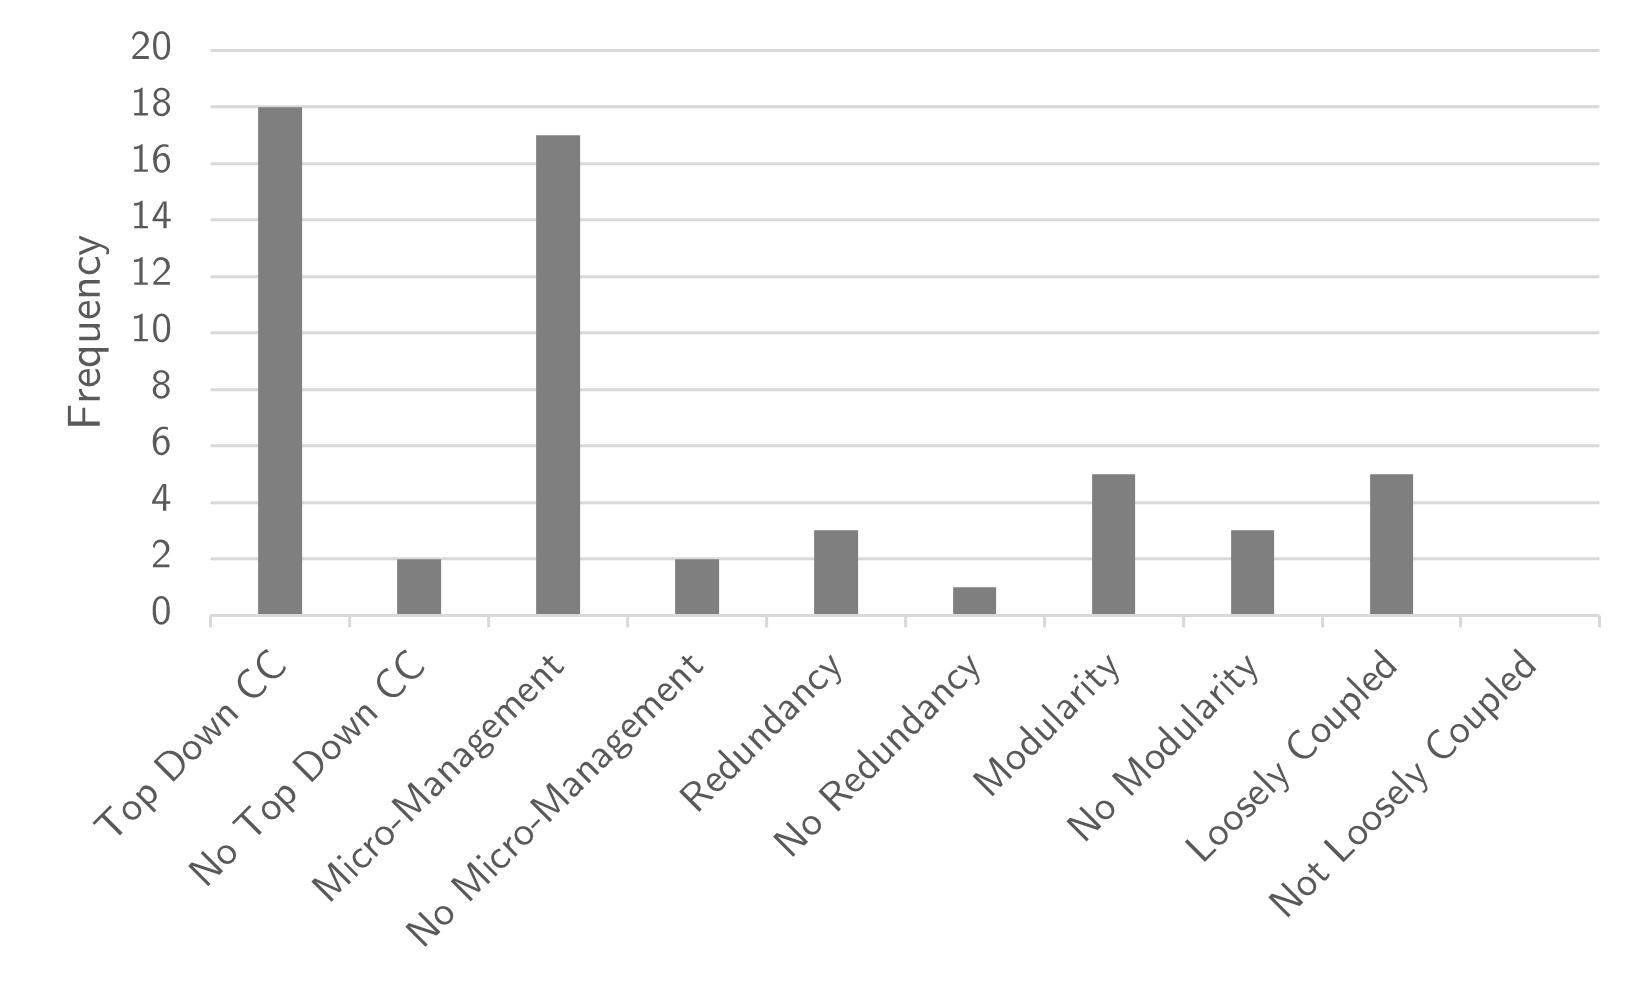
\includegraphics[width=0.95\linewidth]{images/attenuate_frequency}
		\caption[Attenuate variety frequency]{Attenuate variety frequency}
		\label{fig:attenuatefrequency}
	\end{subfigure}%
	\begin{subfigure}[H]{0.5\textwidth}
		\centering
		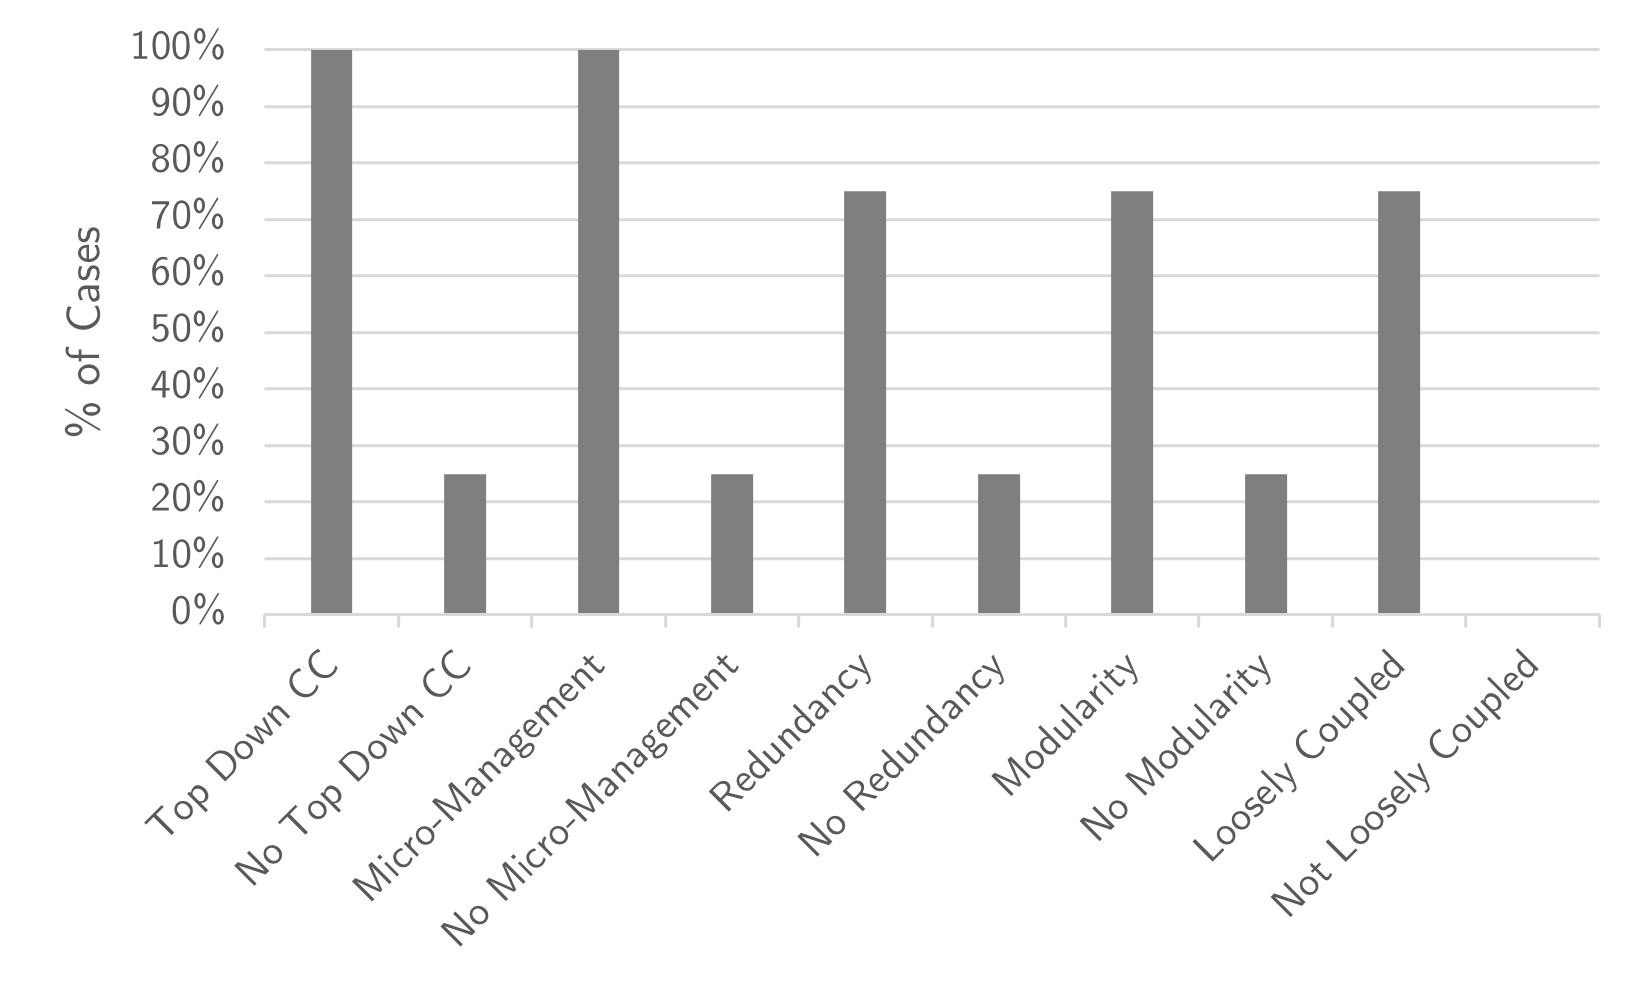
\includegraphics[width=0.95\linewidth]{images/attenuate_cases}
		\caption[Attenuate variety \% of cases]{Attenuate variety \% of cases}
		\label{fig:attenuatecases}
	\end{subfigure}
	\caption[Interview results attenuate variety]{Interview results attenuate variety}
	\label{fig:interviewattenuatevariety}
\end{figure}
E.g. a missing law with the introduction of electric steps (\cref{sec:interviewlocalgovernment}). It is not a bike, not a motorcycle or a car. The electric step did not fit into the current laws and regulations. The result was that the policymakers did not approve it and did not even tolerate it until law-making finished. \Cref{fig:interviewattenuatevariety} also shows that both \textit{\gls{modularity}} and \textit{\gls{looselycoupled}} scored somewhat because the \gls{ps} consists of many subsystems. Every subsystem has a clear goal and a reason to exist. For E.g. local tax offices have the goal of collecting local taxes, while the social services are in charge of paying benefits. Communication between those subsystems is going through standardised interfaces and is predictable. Although \gls{redundancy} is almost non-existent. Every subsystem has its particular goal and reason to exist and cannot take on public tasks another subsystem is performing (\cref{sec:interviewlocalgovernment}).
\subsection{Interview results on amplified variety}
\label{sub:interviewresultsaplified}
\begin{figure}[H]
	\centering
	\begin{subfigure}[H]{0.5\textwidth}
		\centering
		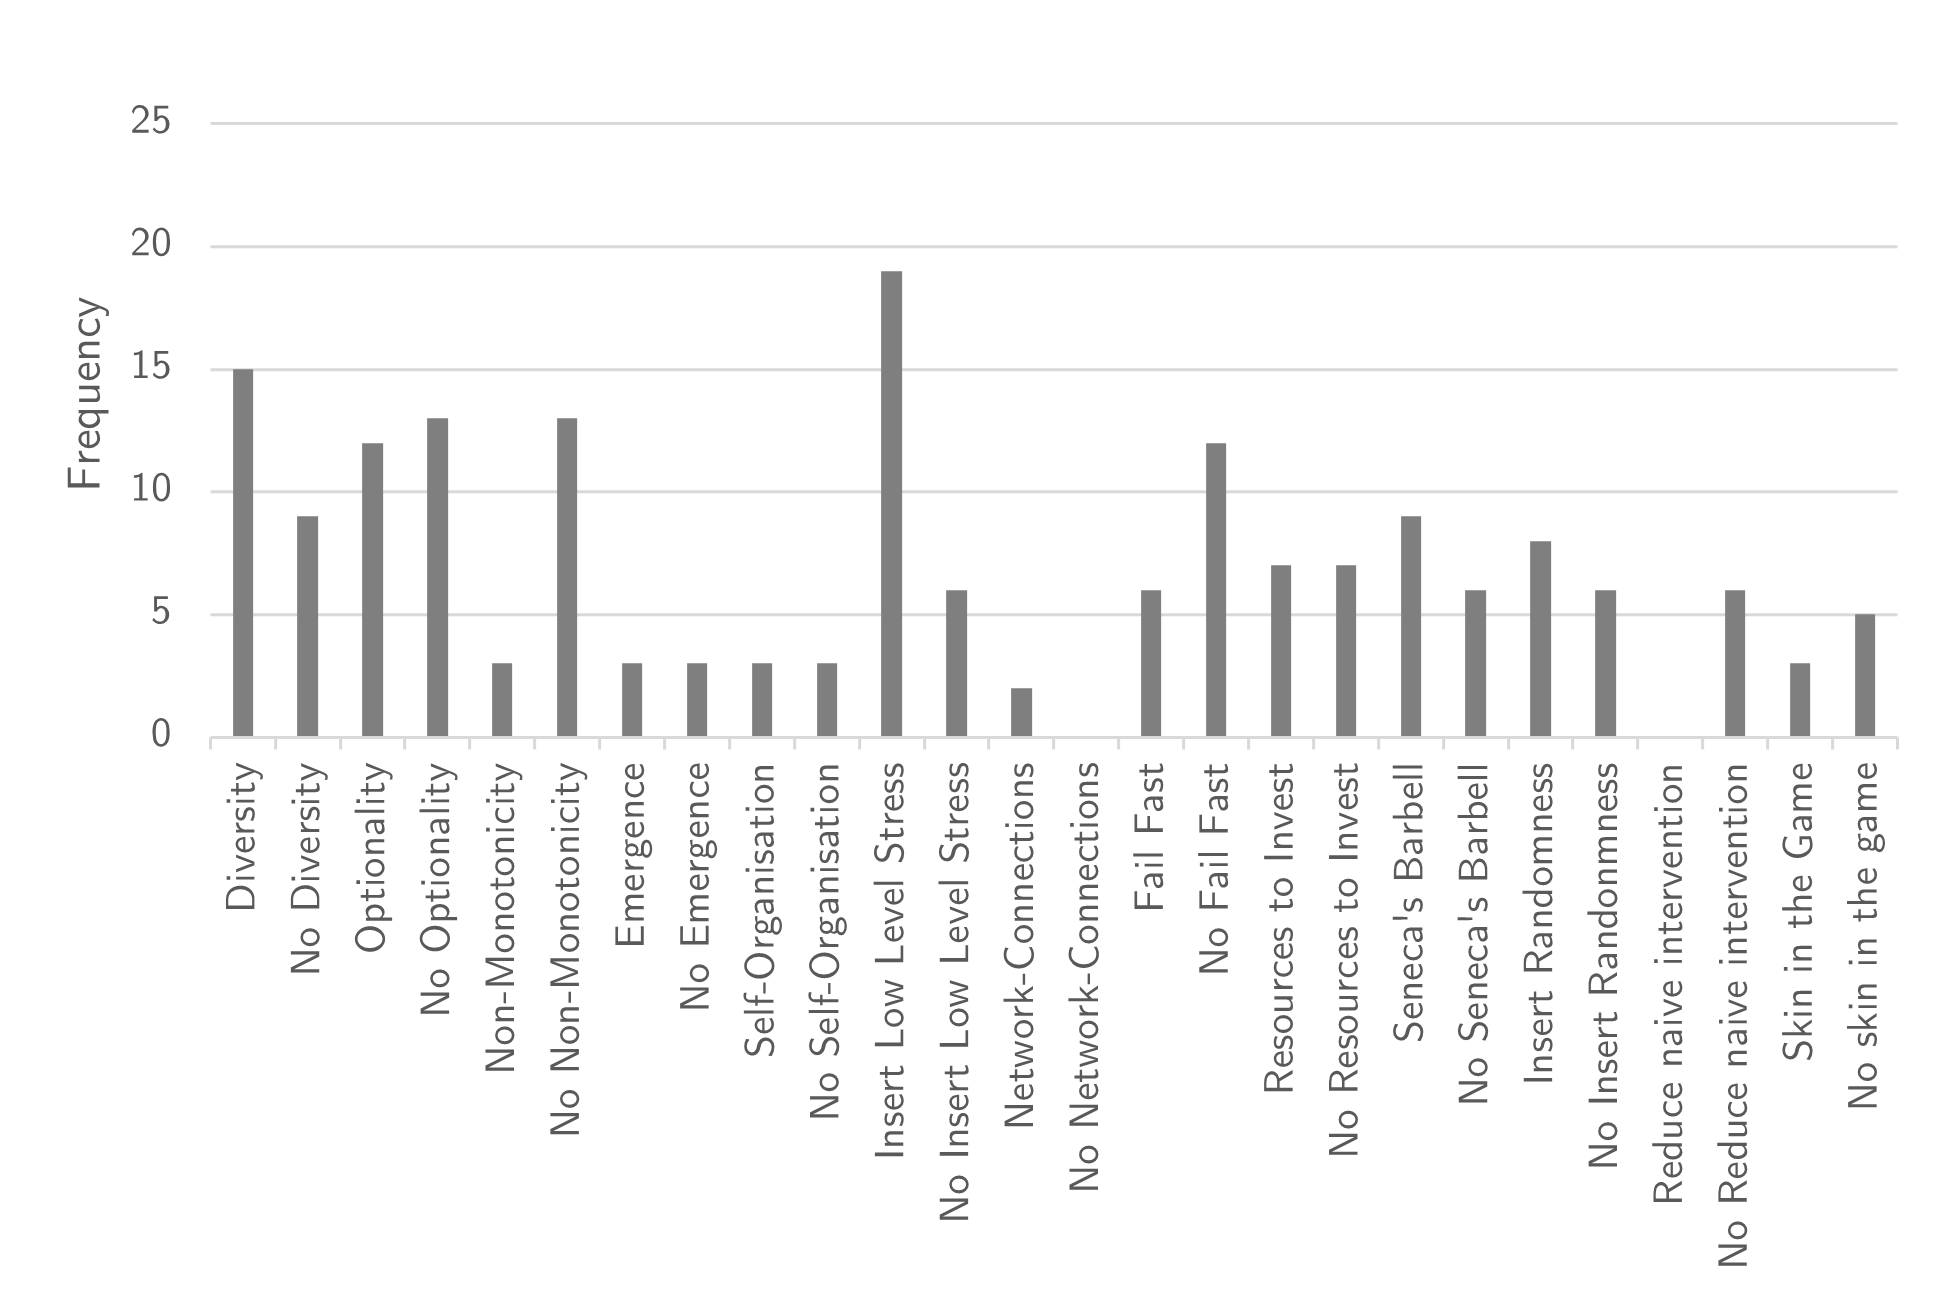
\includegraphics[width=0.95\linewidth]{images/amplified_frequency}
		\caption[Amplified variety frequency]{Amplified variety frequency}
		\label{fig:amplifiedfrequency}
	\end{subfigure}%
	\begin{subfigure}[H]{0.5\textwidth}
		\centering
		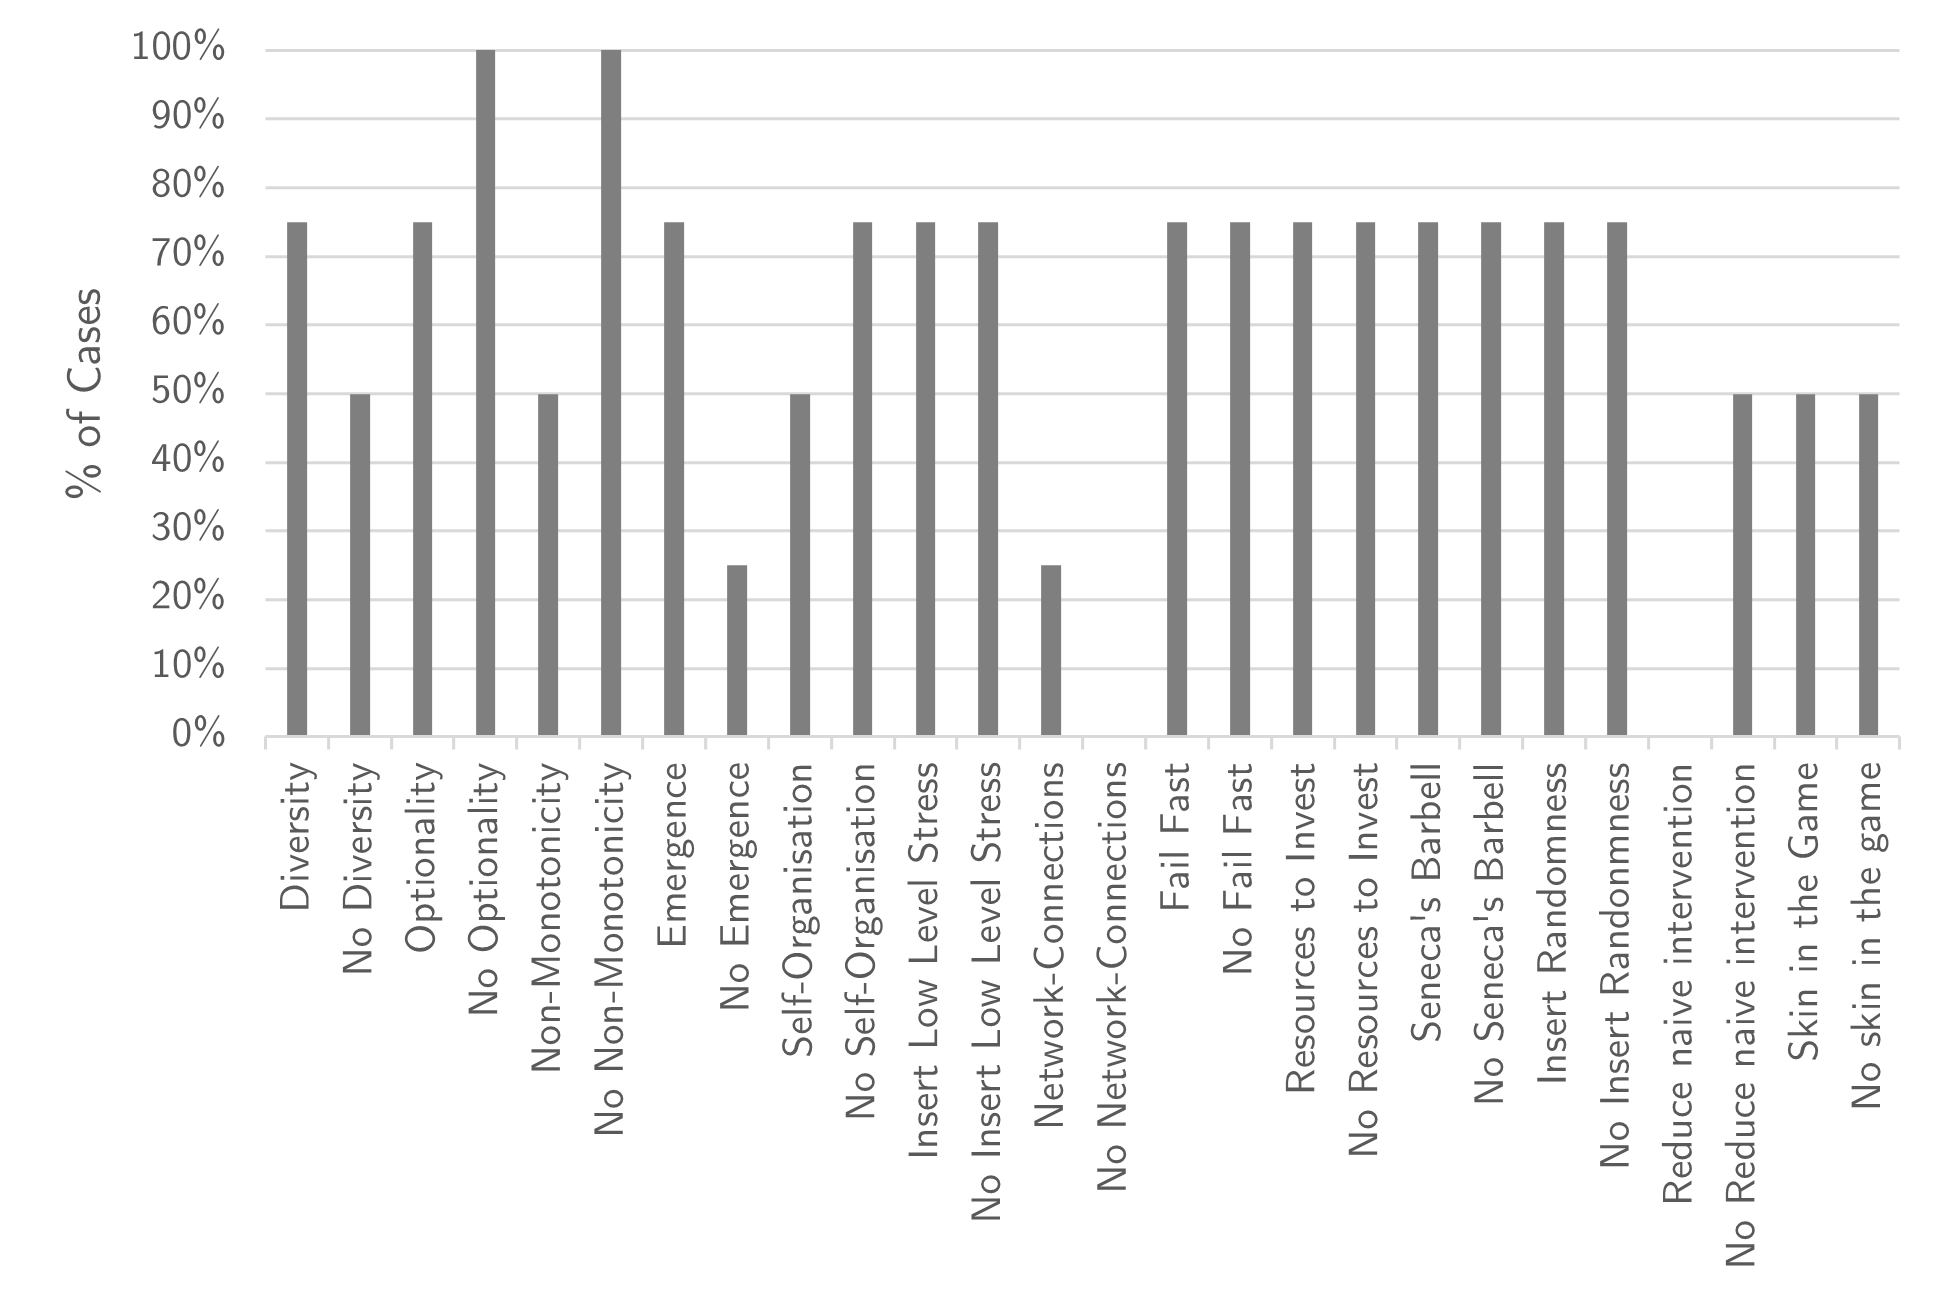
\includegraphics[width=0.95\linewidth]{images/amplified_cases}
		\caption[Amplified variety \% of cases]{Amplified variety \% of cases}
		\label{fig:amplifiedcases}
	\end{subfigure}
	\caption[Interview results amplified variety]{Interview results amplified variety}
	\label{fig:interviewamplifiedvariety}
\end{figure}

No optionality and no-monotonicity


One interviewee stated that the \gls{ps} should be in a permanent crisis situation to get things done.

The end goal is not very clear with \gls{agile} working. It is unclear how the public money is spent on precisely what. 



There is no risk appetite. Everything must be known and explainable in advance. If it is found that the procedures are not used, it can result in political consequences later on. Afterwards, positive lessons learned are not used to make adjustments within the public sector. Experimentation is (almost) not possible.

\subsection{Interview results on Learning organisation}
\label{sub:interviewresultslearning}
\begin{figure}[H]
	\centering
	\begin{subfigure}[H]{0.5\textwidth}
		\centering
		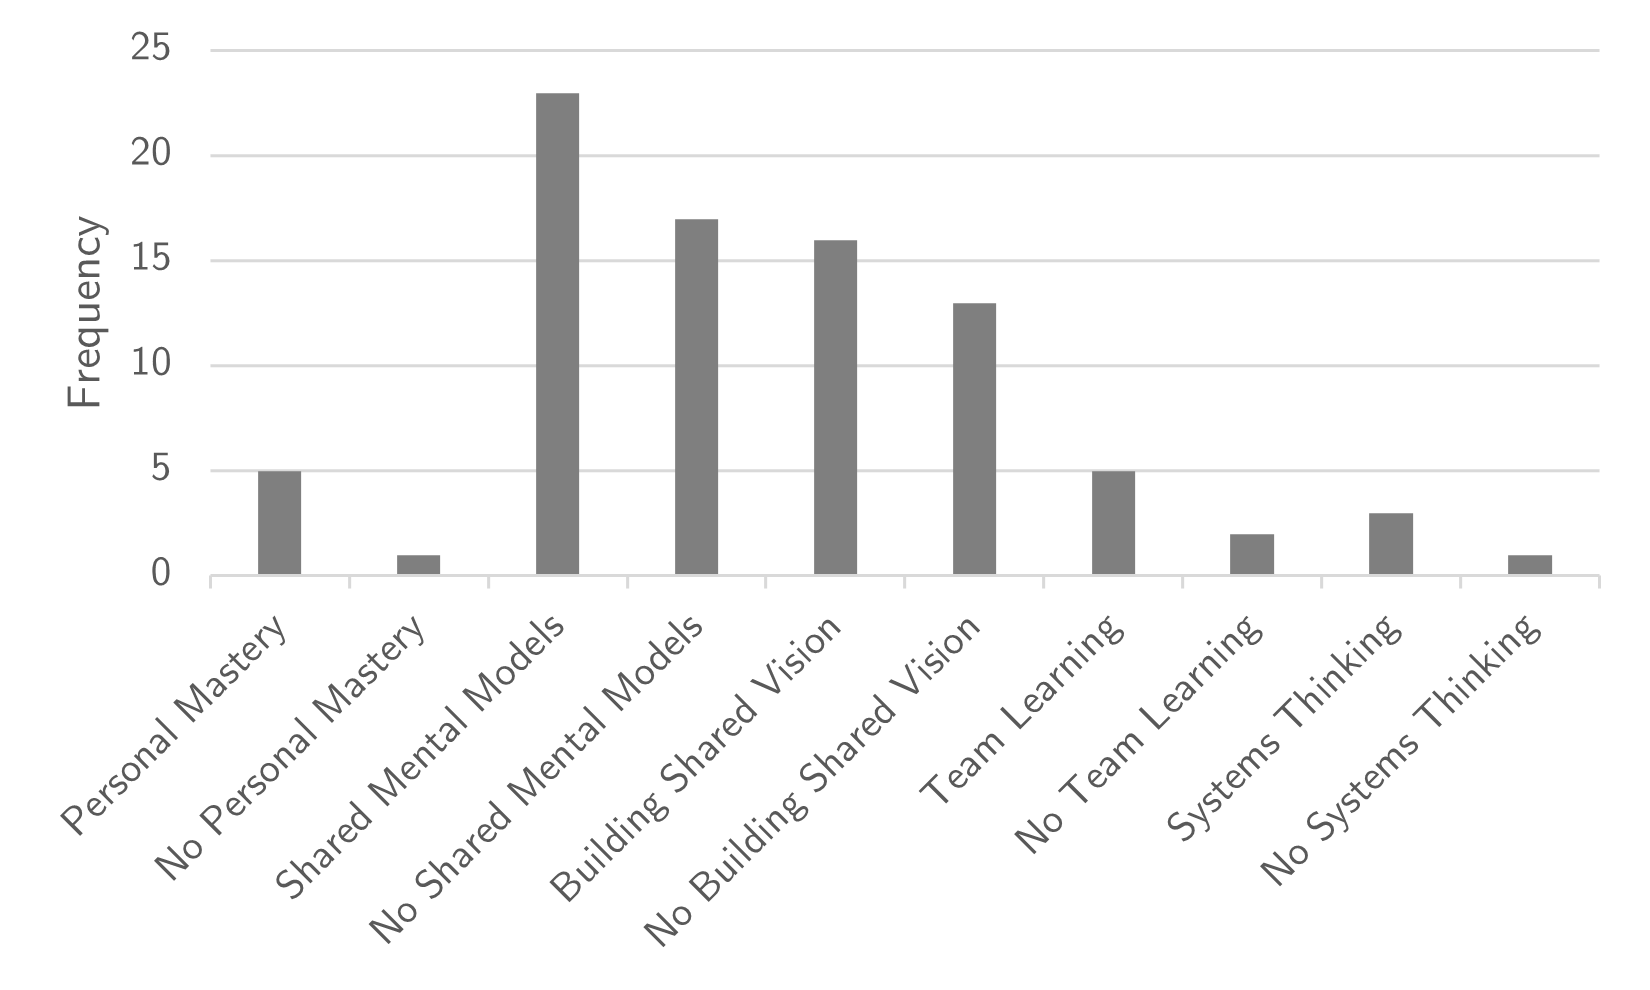
\includegraphics[width=0.95\linewidth]{images/learningorganisation_frequency}
		\caption{Learning organisation Frequency}
		\label{fig:learningfrequency}
	\end{subfigure}%
	\begin{subfigure}[H]{0.5\textwidth}
		\centering
		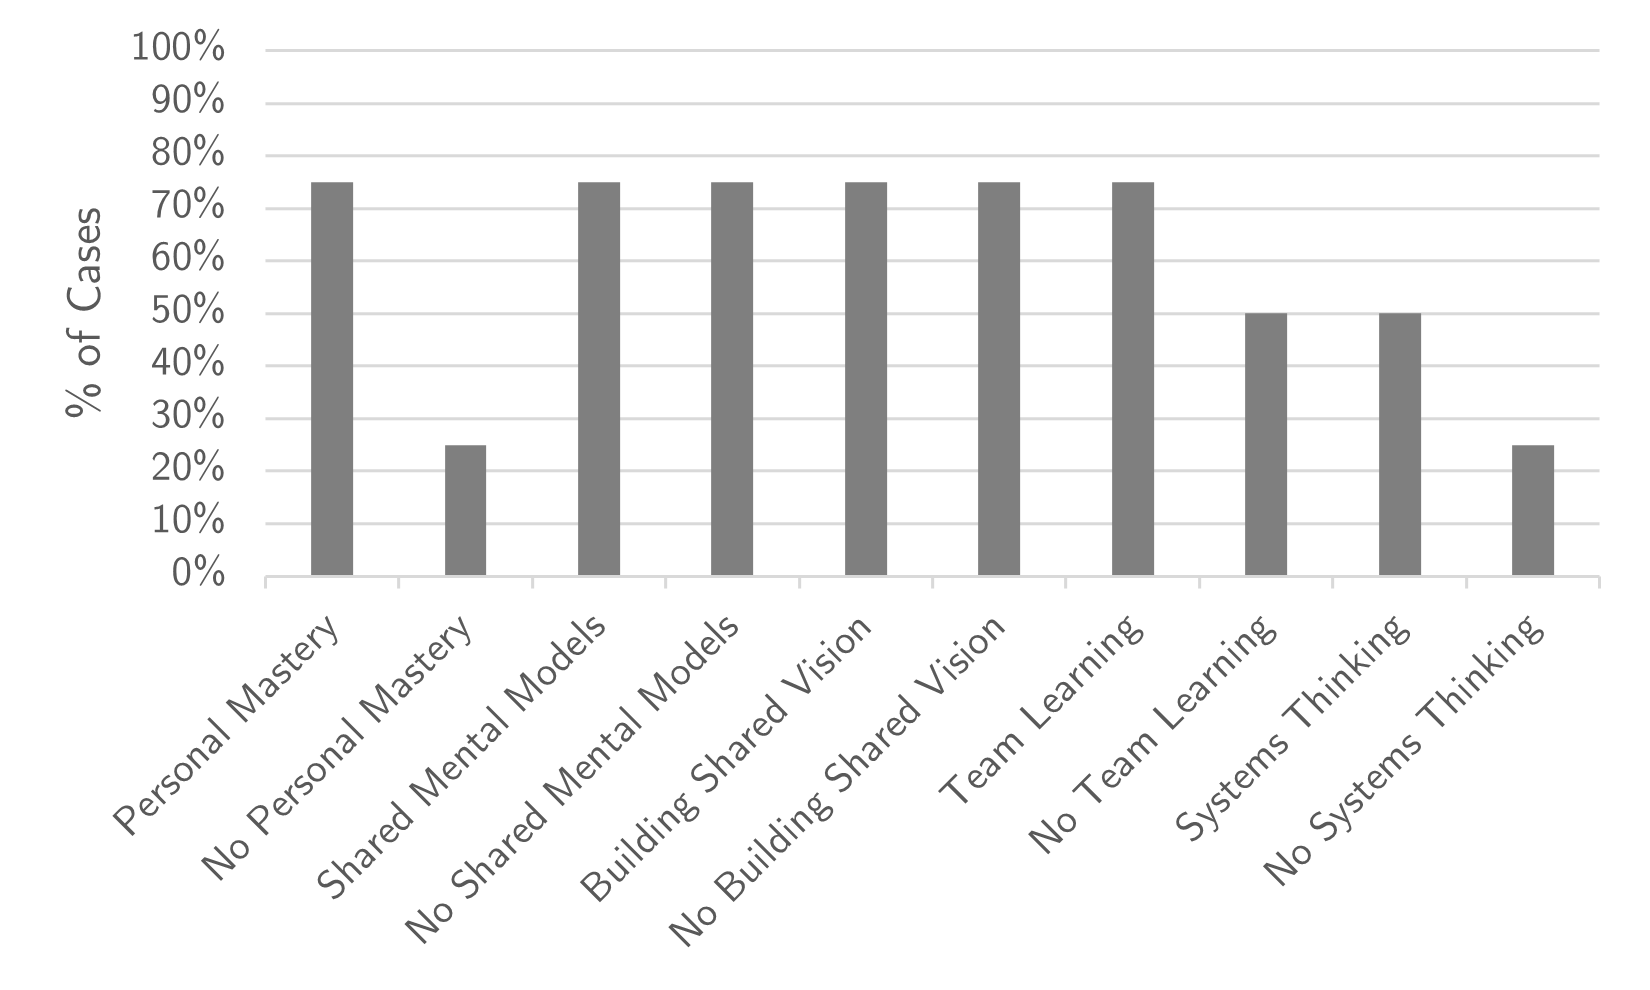
\includegraphics[width=0.95\linewidth]{images/learningorganisation_cases}
		\caption{Learning organisation \% of Cases}
		\label{fig:learningcases}
	\end{subfigure}
	\caption{Interview results Learning organisation}
	\label{fig:interviewlearningorganisation}
\end{figure}

\subsection{Interview results on Enterprise Architecture schools of thought}
\label{sub:interviewresultseaschools}
\begin{figure}[H]
	\centering
	\begin{subfigure}[H]{0.5\textwidth}
		\centering
		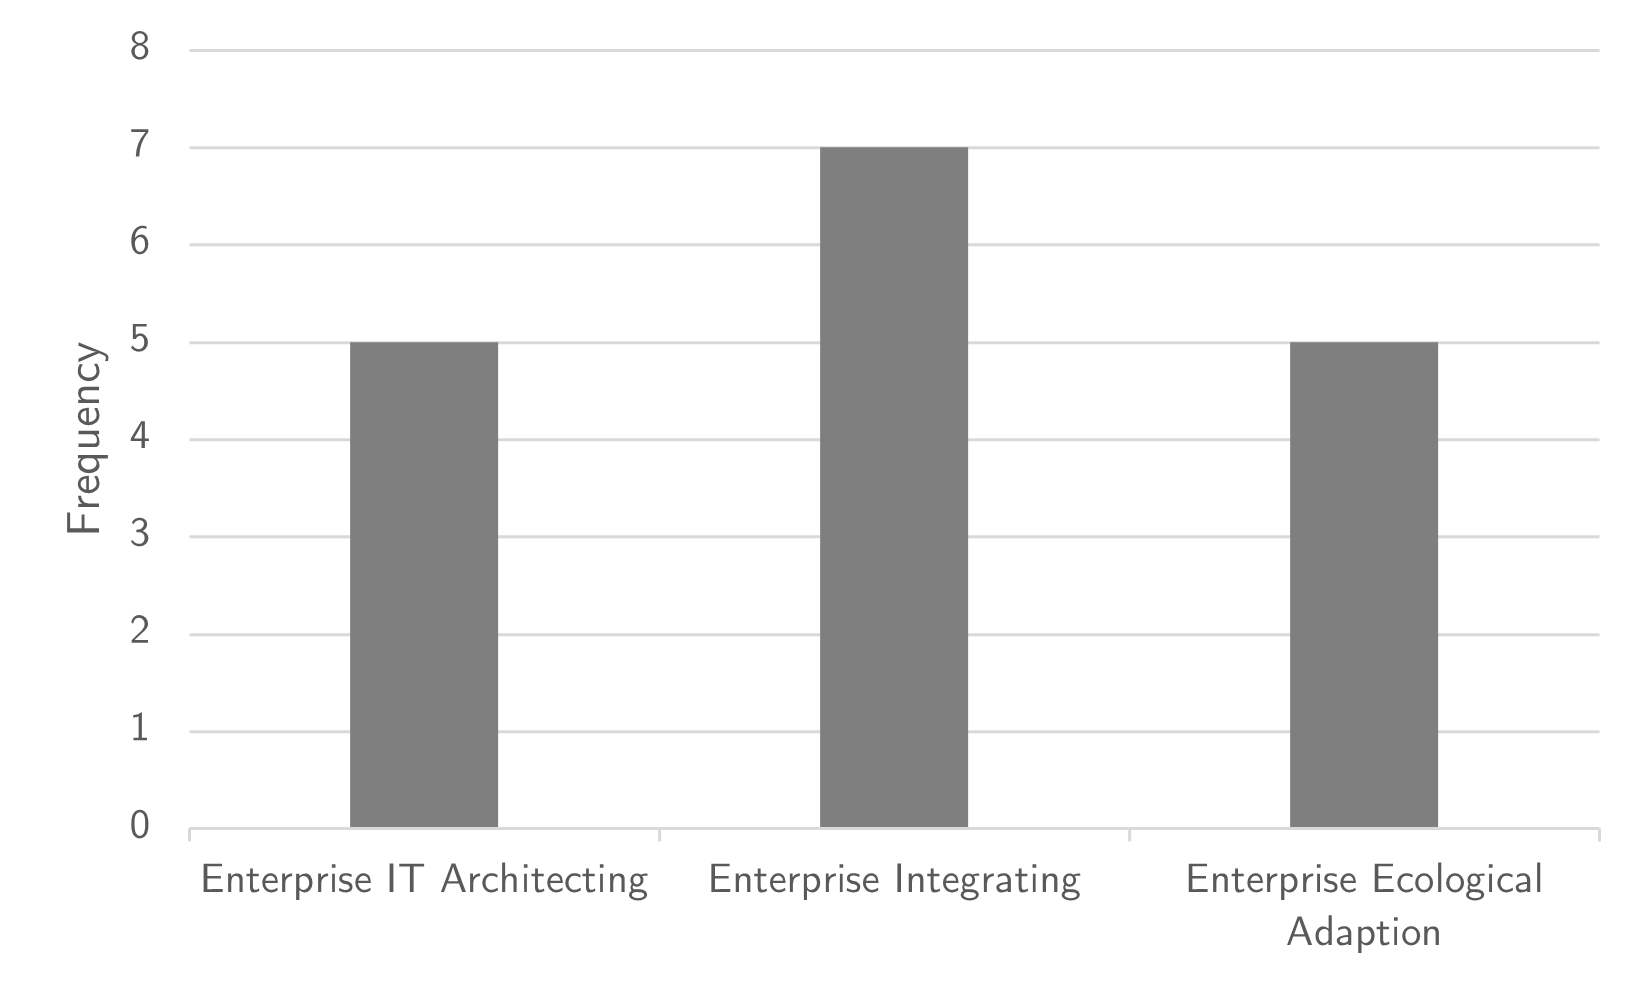
\includegraphics[width=0.95\linewidth]{images/easchools_frequency}
		\caption{Enterprise Architecture Schools of thought Frequency}
		\label{fig:easchoolsfrequency}
	\end{subfigure}%
	\begin{subfigure}[H]{0.5\textwidth}
		\centering
		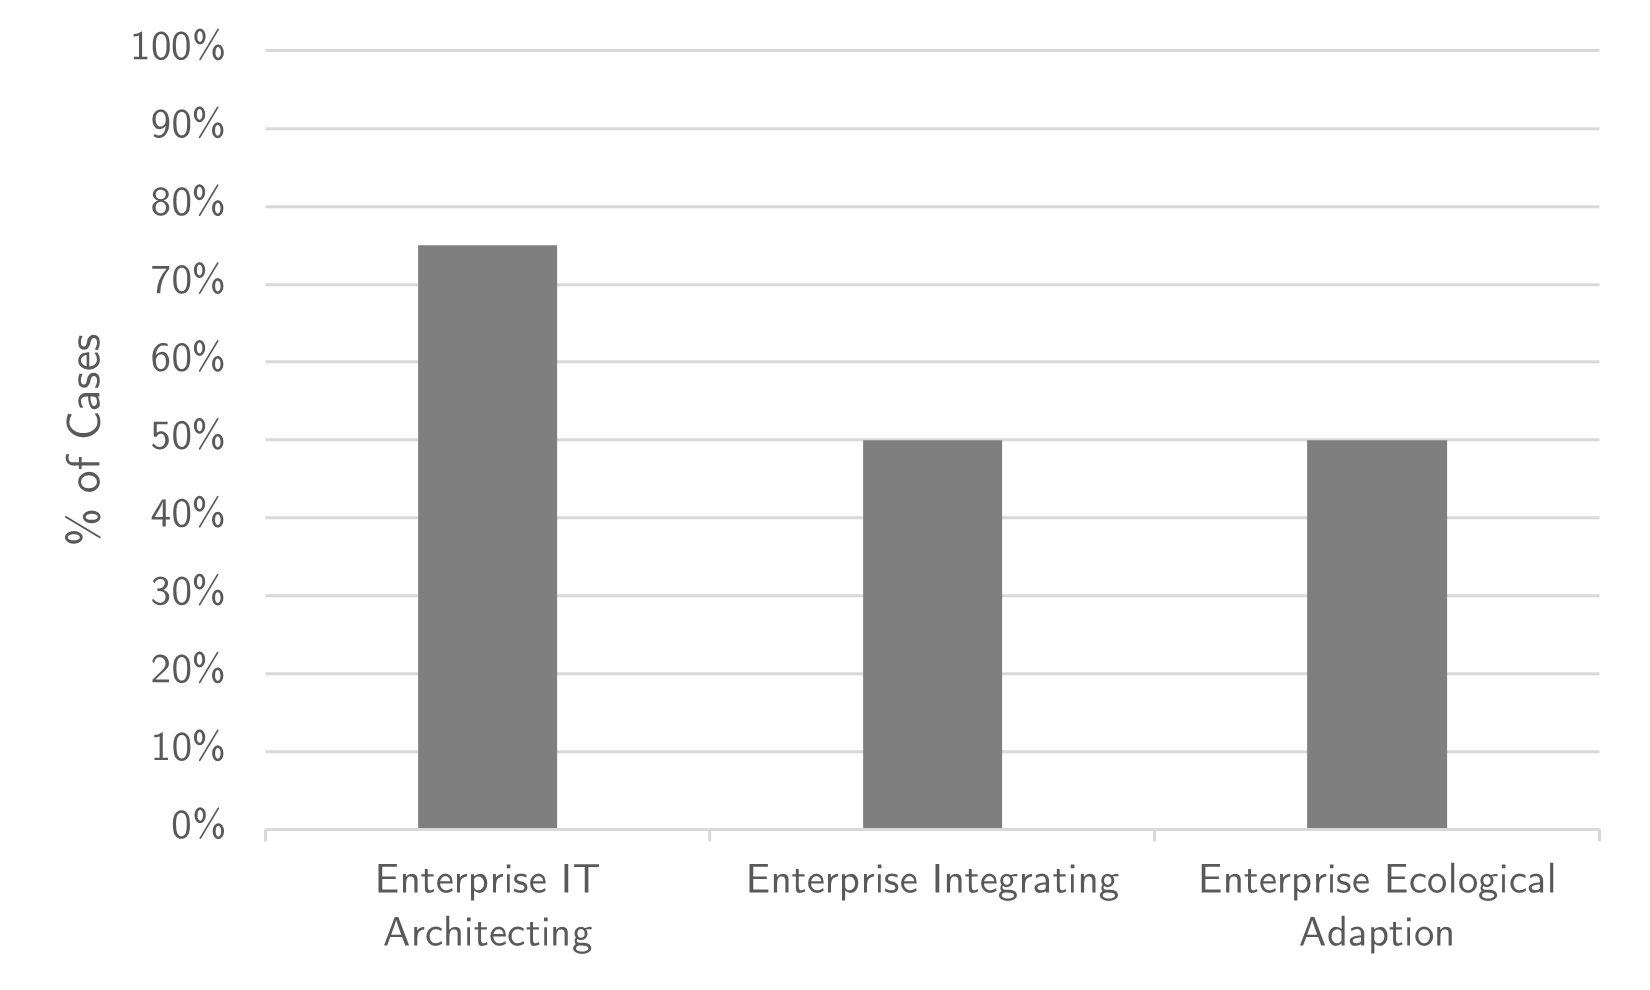
\includegraphics[width=0.95\linewidth]{images/easchools_cases}
		\caption{Enterprise Architecture Schools of thought \% of Cases}
		\label{fig:easchoolscases}
	\end{subfigure}
	\caption{Interview results Enterprise Architecture schools of thought}
	\label{fig:easchoolsantifragile}
\end{figure}



What we have to do in the public sector depends on the political decision making within the period of governing (four years until new elections). \acrshort{ea} is at the end of the chain of administrative decision-making.

\subsection{Interview results on possible new attributes}
\begin{figure}[H]
	\centering
	\begin{subfigure}[H]{0.5\textwidth}
		\centering
		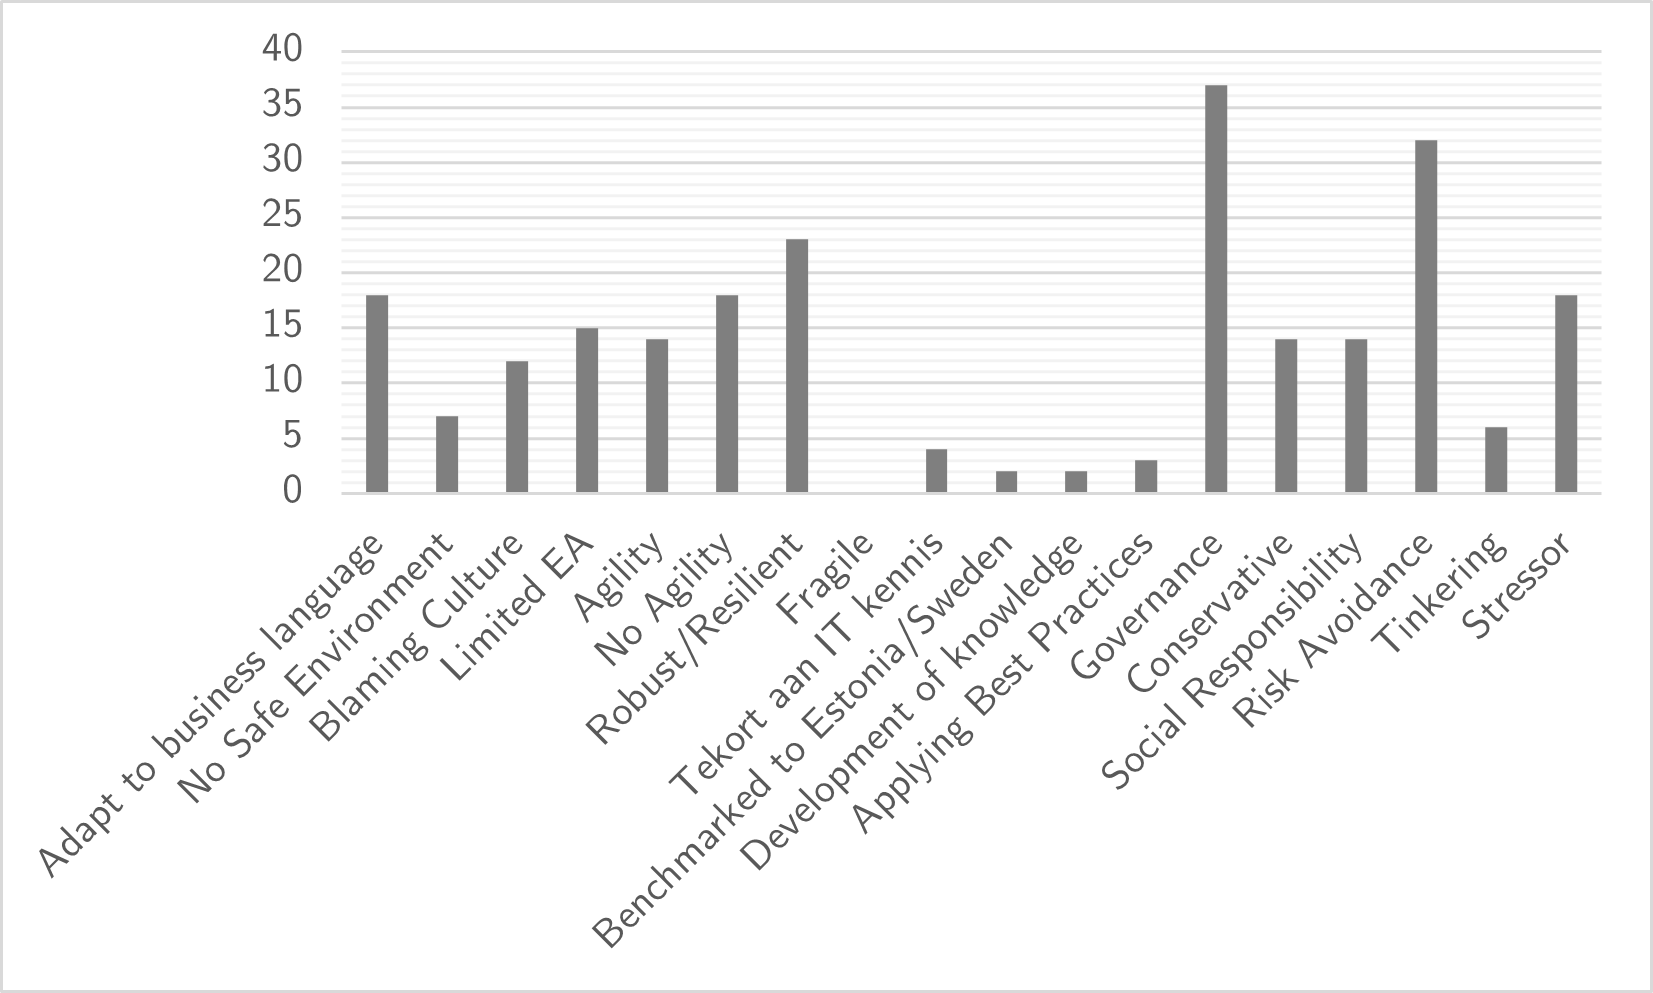
\includegraphics[width=0.95\linewidth]{images/findings_frequency}
		\caption{Findings Frequency}
		\label{fig:findingsfrequency}
	\end{subfigure}%
	\begin{subfigure}[H]{0.5\textwidth}
		\centering
		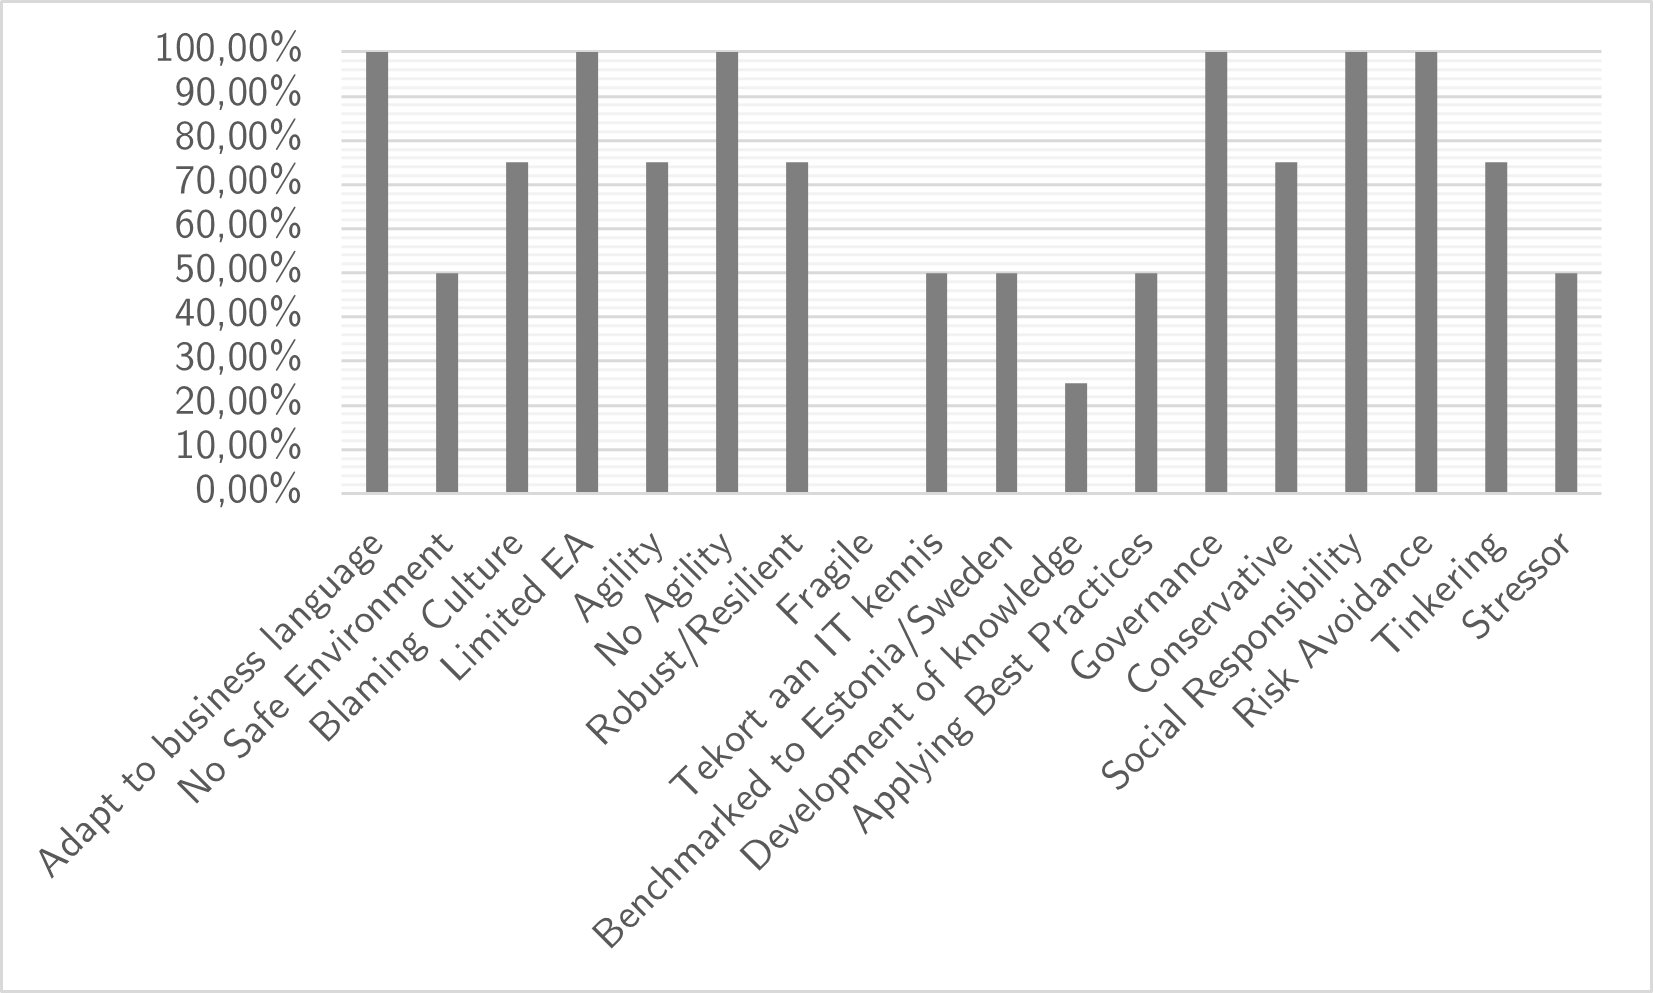
\includegraphics[width=0.95\linewidth]{images/findings_cases}
		\caption{Findings \% of Cases}
		\label{fig:findingscases}
	\end{subfigure}
	\caption{Interview results Findings}
	\label{fig:interviewresultsfindings}
\end{figure}

\section{Qualitative Data Analysis}
\label{sec:dataprep}

\subsection{Merging similar attributes}
\label{sub:merginglabels}
\begin{table}[H]
	\centering
	\resizebox{\textwidth}{!}{%
		\begin{tabular}{p{.05\textwidth}p{.5\textwidth}p{.45\textwidth}}
			\toprule %
			\textbf{Step} & \textbf{Description} & \textbf{Rationale} \\%
			\midrule %
			1	  & Create, positive and negative main categories of Engineering, Systems, CAS, \gls{antifragile}, and Learning organisation. & Need extra categories for merging overarching subjects. \\%
			2     & Merge \gls{agility} into CAS & How \gls{agility} is interpreted is the same as CAS \\%
			3     & Merge tinkering into Learning Organisation & How tinkering is interpreted it is the same as Learning Organisation. \\%
			4     & Merge \gls{robust} and \gls{resilient} into Engineering Resilience & How \gls{robust} and \gls{resilient} is interpreted by interviewees is the same as Engineering Resilience. \\%
			5     & Merge Governance into Engineering Resilience & How Governance is interpreted is the same as \gls{topdowncc} and \gls{micromanagement}. \\%
			6     & Merge Shortage on IT Knowledge into no \gls{resourcestoinvest} & Shortage on IT Knowledge can be interpreted as a resource that is not there \\%
			7     & Merge Applying Best practices into \gls{nonmonotonicity} & Applying Best practices is learning from the past. \\%
			8     & Merge Development of Knowledge into Learning Organisation & Development of Knowledge within an organisation can be seen as the learning capability of an organisation. \\%
			9     & Merge Blaming Culture into No Safe Environment & No Safe Environment is a result of a Blaming Culture. \\%
			10    & Merge Limited \acrshort{ea} into \gls{enterpriseitarchitecting} & Limited \acrshort{ea} is interpreted as the school of thought \gls{enterpriseitarchitecting} \\%
			11    & Merge conservative into Risk Avoidance & Risk Avoidance is a result of conservative \\%
			12	  & Ignored Social Responsibility and Risk Avoidance as \glspl{attribute} as possible success factors & Social Responsibility and Risk Avoidance are attributes of the \gls{ps} and are less relevant as an attribute for \gls{antifragile} and \acrshort{ea}. \\%
			\bottomrule %
		\end{tabular}%
	}%
	\caption{Data preparation - Merging similar labels}
	\label{tab:prepmergingsimilarlabels}%
\end{table}%

\subsection{Normalise frequency of attributes}
\label{sub:normalisefrequency}
To remove (emotional) bias of interviewees the frequency is normalised by only counting the occurrence of an attribute once per question per interview.
\begin{table}[H]
	\centering
	\resizebox{\textwidth}{!}{%
		\begin{tabular}{p{.05\textwidth}p{.5\textwidth}p{.45\textwidth}}
			\toprule %
			\textbf{Step} & \textbf{Description} & \textbf{Rationale} \\%
			\midrule %
			1		&	Count the presence of an \gls{attribute} only once per question per interview. & Removing (emotional) bias. With seven main questions the score of an \gls{attribute} can have a maximum of seven per interview. With four conducted interviews the maximum score of an \gls{attribute} is twenty-eight. \\%
			\bottomrule %
		\end{tabular}%
	}%
	\caption[Data preparation - Normalise frequency of attributes]{Data preparation - Normalise frequency of attributes}
	\label{tab:normalisefrequency}%
\end{table}%

\subsection{Normalise score of attributes}
\label{sub:normalisescore}

\begin{table}[H]
	\centering
	\resizebox{\textwidth}{!}{%
		\begin{tabular}{p{.05\textwidth}p{.5\textwidth}p{.45\textwidth}}
			\toprule %
			\textbf{Step} & \textbf{Description} & \textbf{Rationale} \\%
			\midrule %
			1		&	Add for every lonely negative a 0 positive & Looking for \glspl{attribute} that can be a success factor after normalisation. \\%
			2		&	\Gls{attribute} score is Positive value - Negative value & Bringing the values back to the found \glspl{attribute}. \\%
			3		&	Split up between literature found, \acrshort{ea} and new findings & Categorise. For the literature found there are 2 corners of the triangle. \acrshort{ea} is a different subject than antifragile. The newly found do not have a data point in the literature study of the triangulation. \\%
			\bottomrule %
		\end{tabular}%
	}%
	\caption[Data preparation - Normalise score of attributes]{Data preparation - Normalise score of attributes}
	\label{tab:prepnormalise}%
\end{table}%

\subsection{Filter attributes on threshold 75\% of Cases}
\label{sub:filteronthresholdcases}
\begin{table}[H]
	\centering
	\resizebox{\textwidth}{!}{%
	\begin{tabular}{p{.05\textwidth}p{.5\textwidth}p{.45\textwidth}}
		\toprule %
		\textbf{Step} & \textbf{Description} & \textbf{Rationale} \\%
		\midrule %
		1     & Select labels where \% case is 75\% or more & When three interviewees mentioned the attribute it could be a label of significance (Triangulation) \\%
		\bottomrule
	\end{tabular}%
	}%
	\caption{Data preparation - Filter attributes on threshold 75\% of Cases}
	\label{tab:prepselectcases}%
\end{table}%

\section{Results of Qualitative Data Analysis}

\subsection{Results of QDA Attenuate and Amplified variety}
\label{sub:resultsqdavariety}
\begin{figure}[H]
	\centering
	\begin{subfigure}[H]{0.475\textwidth}
		\centering
		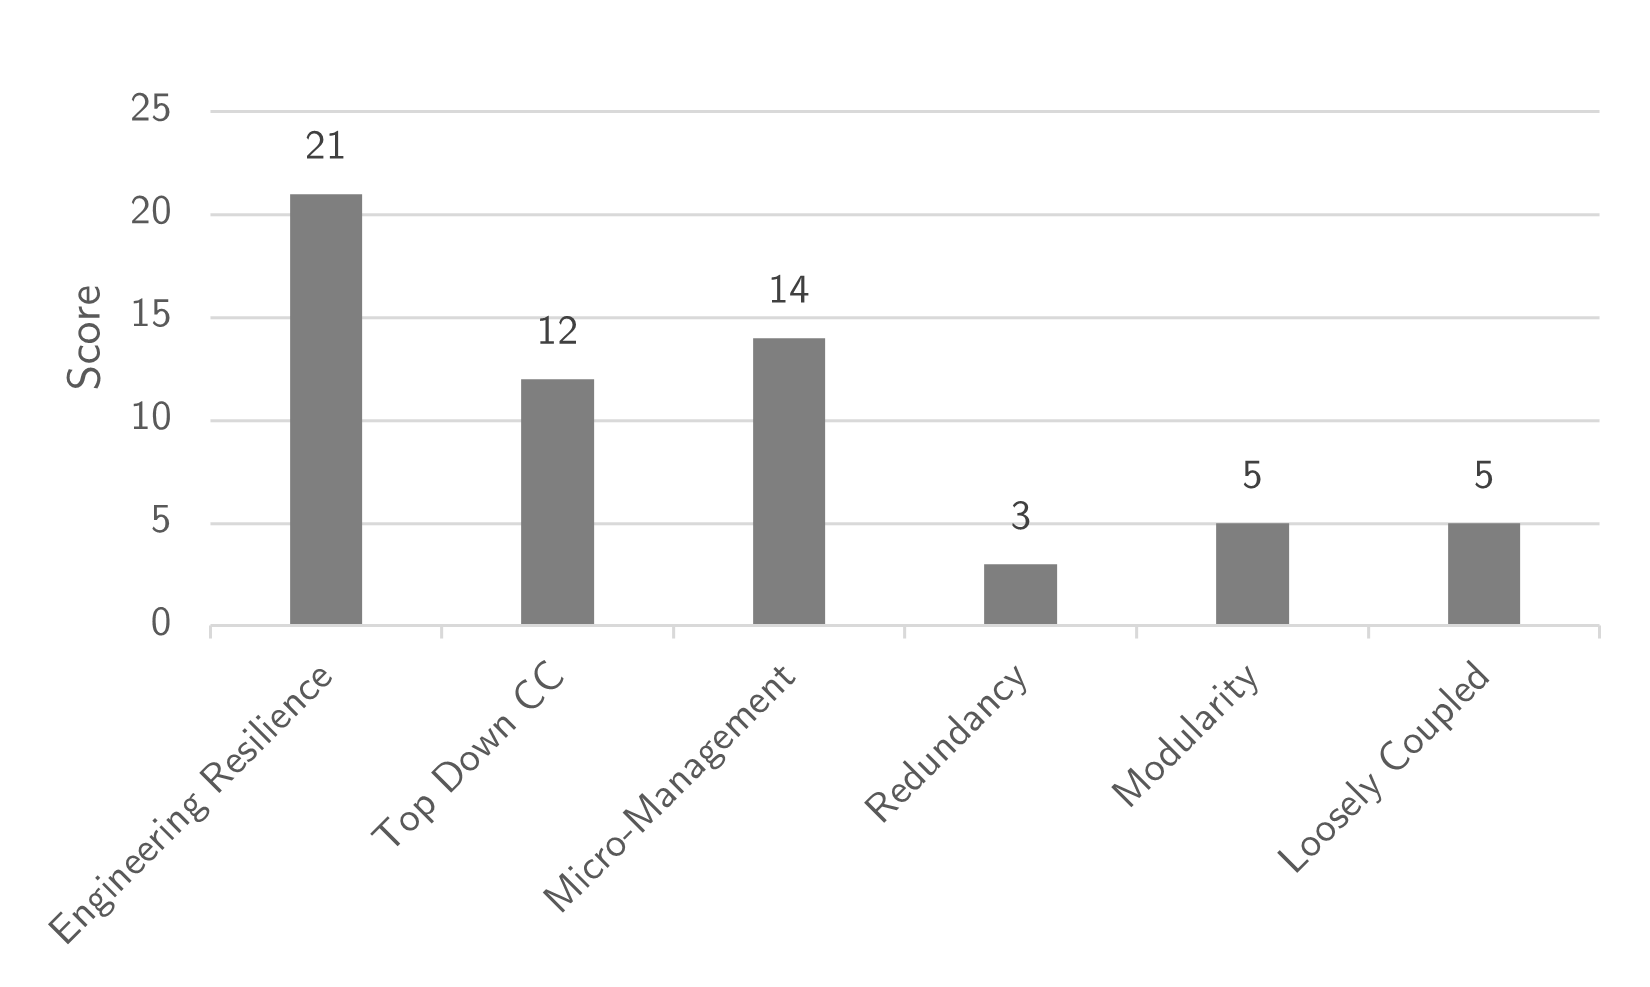
\includegraphics[width=\textwidth]{images/qdaattenuate}
		\caption{QDA Attenuate variety}
		\label{fig:qdaattenuate}
	\end{subfigure}%
\hfill
	\begin{subfigure}[H]{0.475\textwidth}
		\centering
		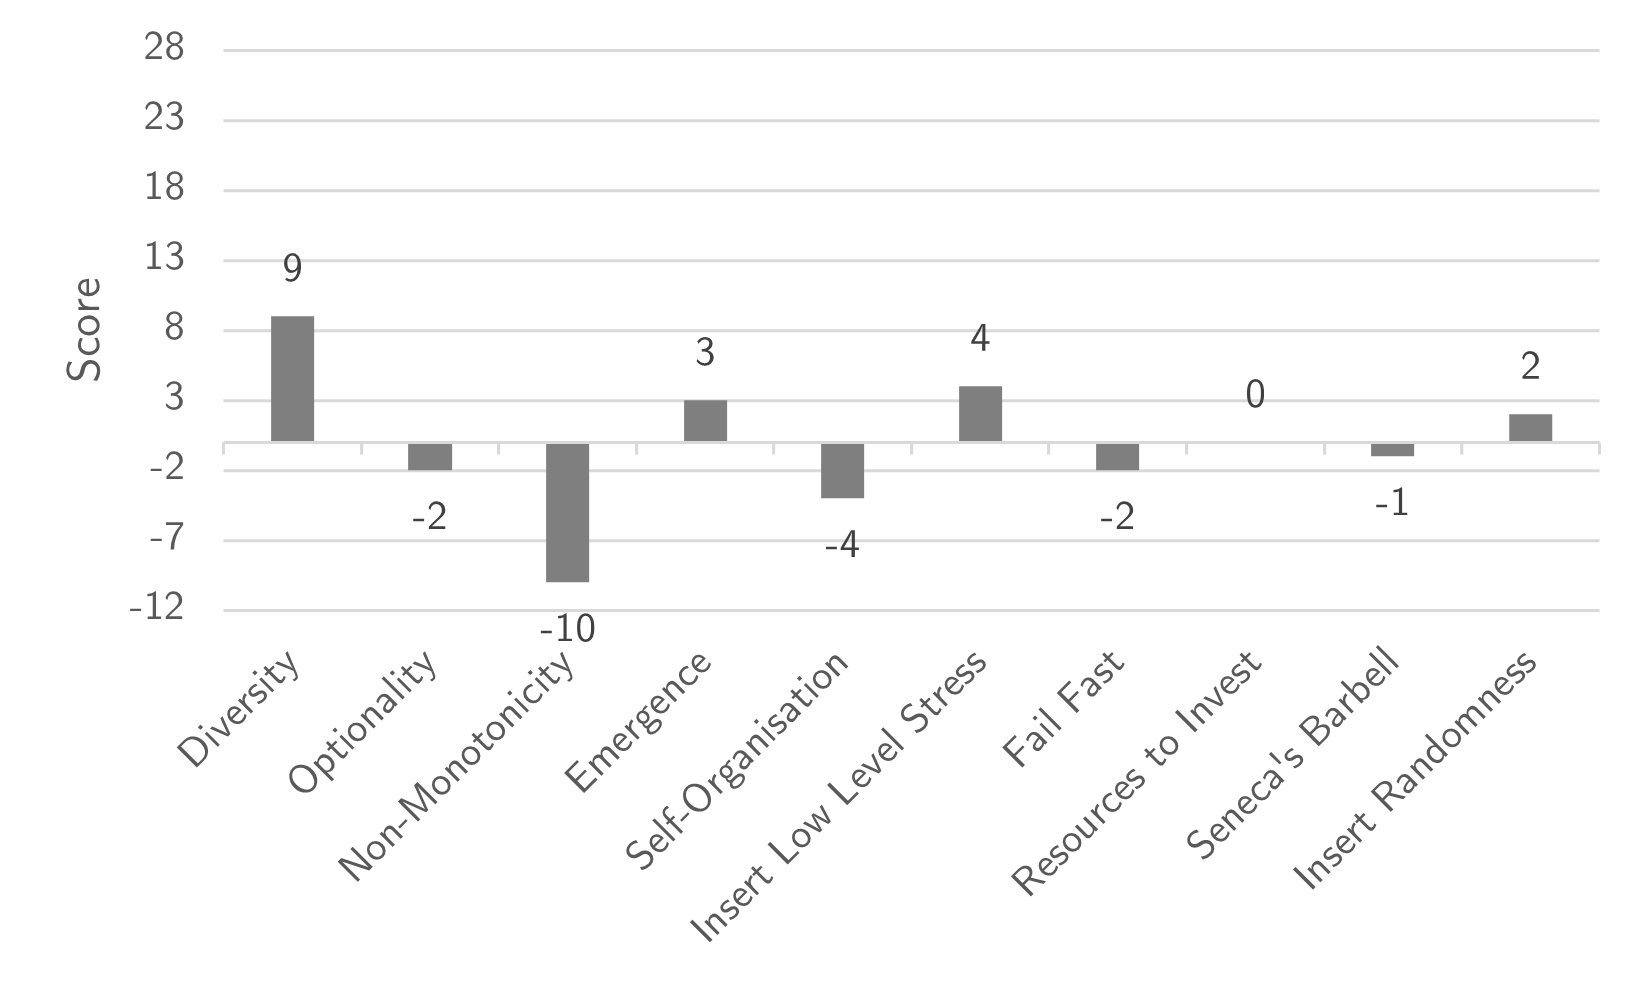
\includegraphics[width=\textwidth]{images/qdaamplify}
		\caption{QDA Amplified variety}
		\label{fig:qdaamplified}
	\end{subfigure}
	\caption{Results of QDA Attenuate and Amplified variety}
	\label{fig:resultsofqdavariety}
\end{figure}

\subsection{Results of QDA Learning organisation and EA school of thought}
\label{sub:resultsqdalearningandea}
\begin{figure}[H]
	\centering
	\begin{subfigure}[H]{0.475\textwidth}
		\centering
		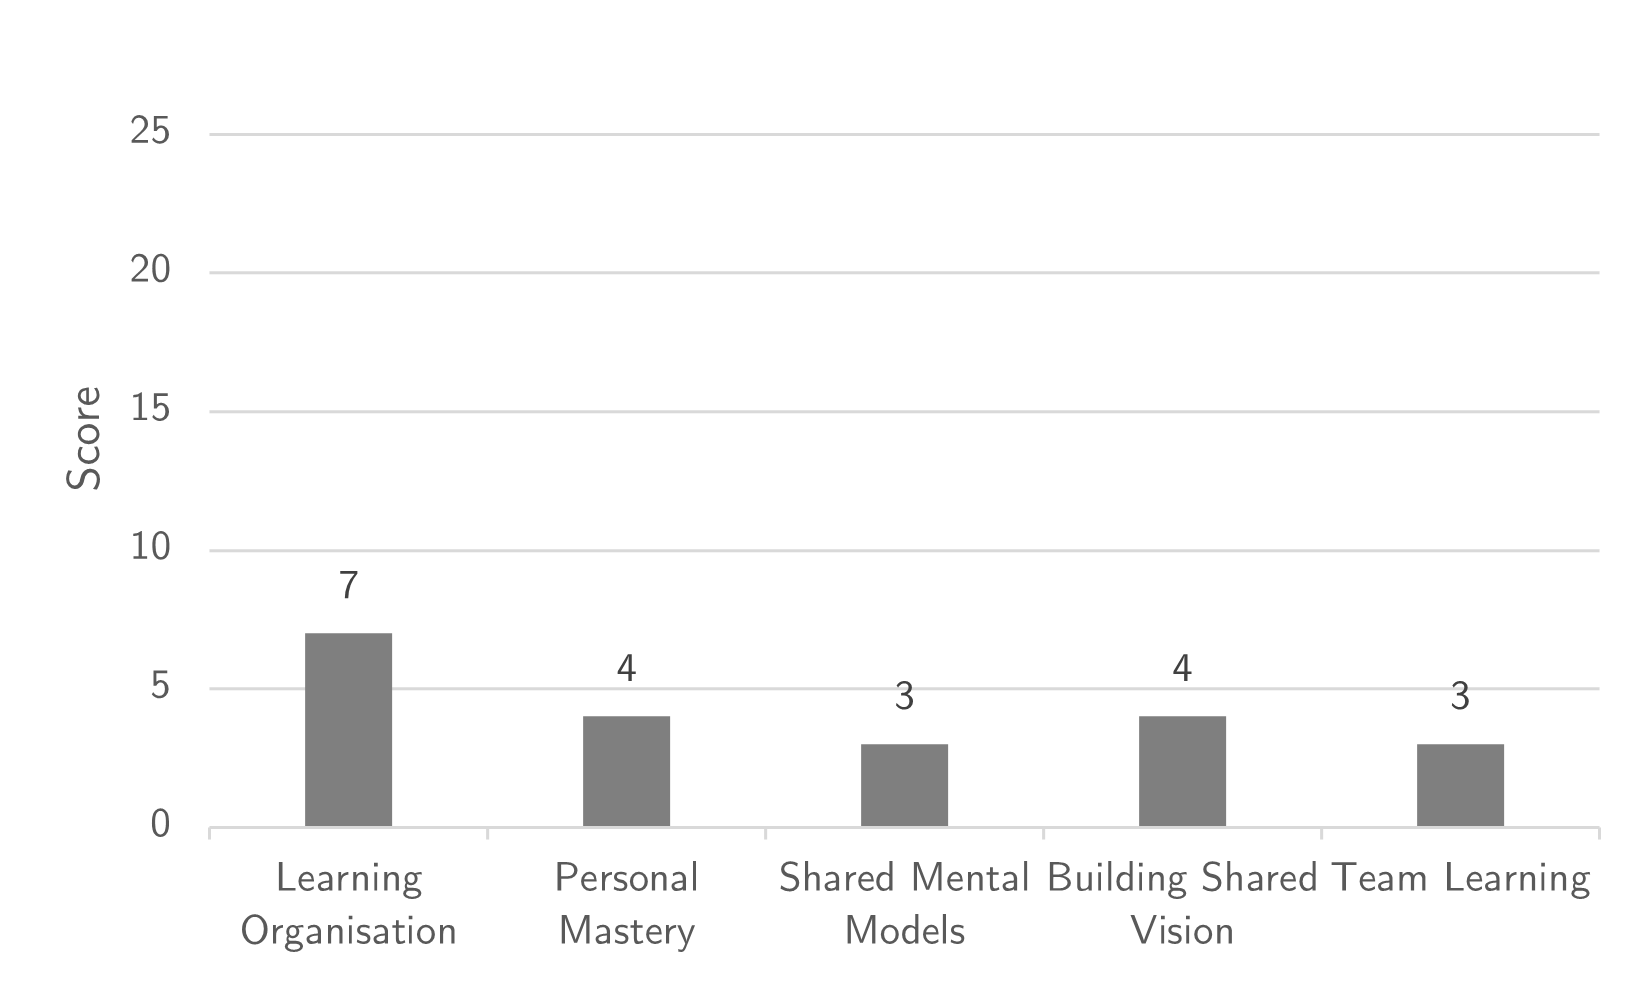
\includegraphics[width=\textwidth]{images/qdalearningorganisation}
		\caption{QDA Learning organisation}
		\label{fig:qdalearning}
	\end{subfigure}%
\hfill
	\begin{subfigure}[H]{0.475\textwidth}
		\centering
		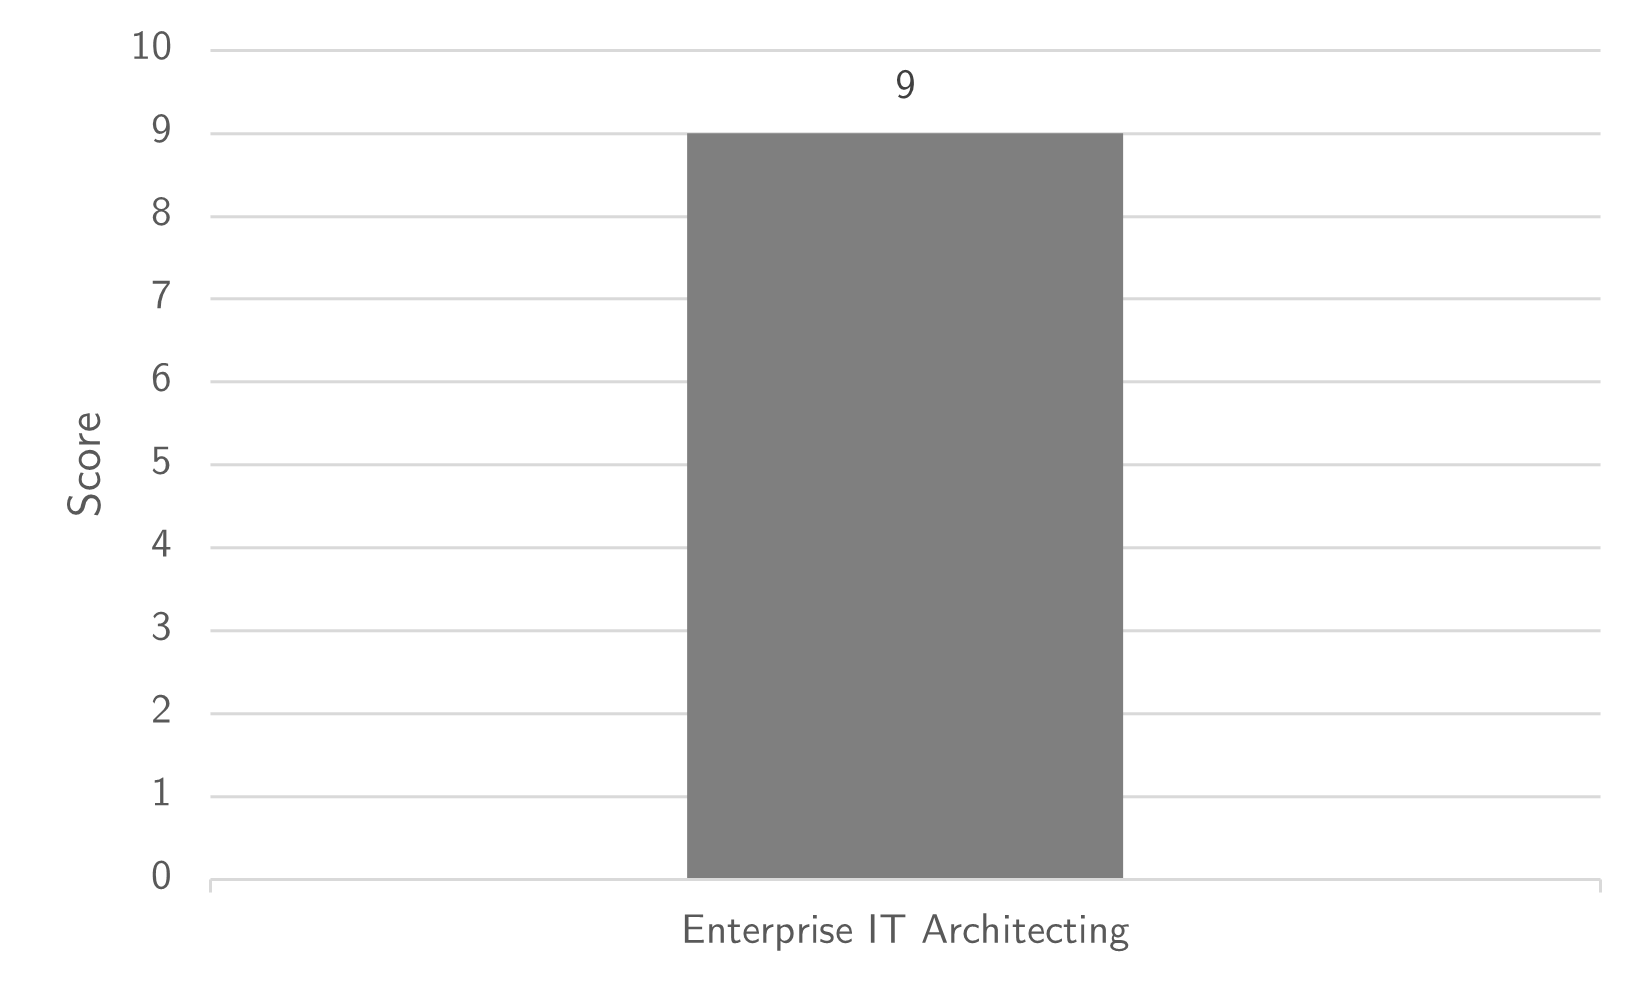
\includegraphics[width=\textwidth]{images/qdaeaschool}
		\caption{QDA EA school of thought}
		\label{fig:qdaea}
	\end{subfigure}
	\caption{Results of QDA Learning organisation and EA school of thought}
	\label{fig:resultsofqda}
\end{figure}

\subsection{Results of QDA of new possible attributes}
\label{sub:resultsqdanewaatributes}
\begin{figure}[H]
	\centering
	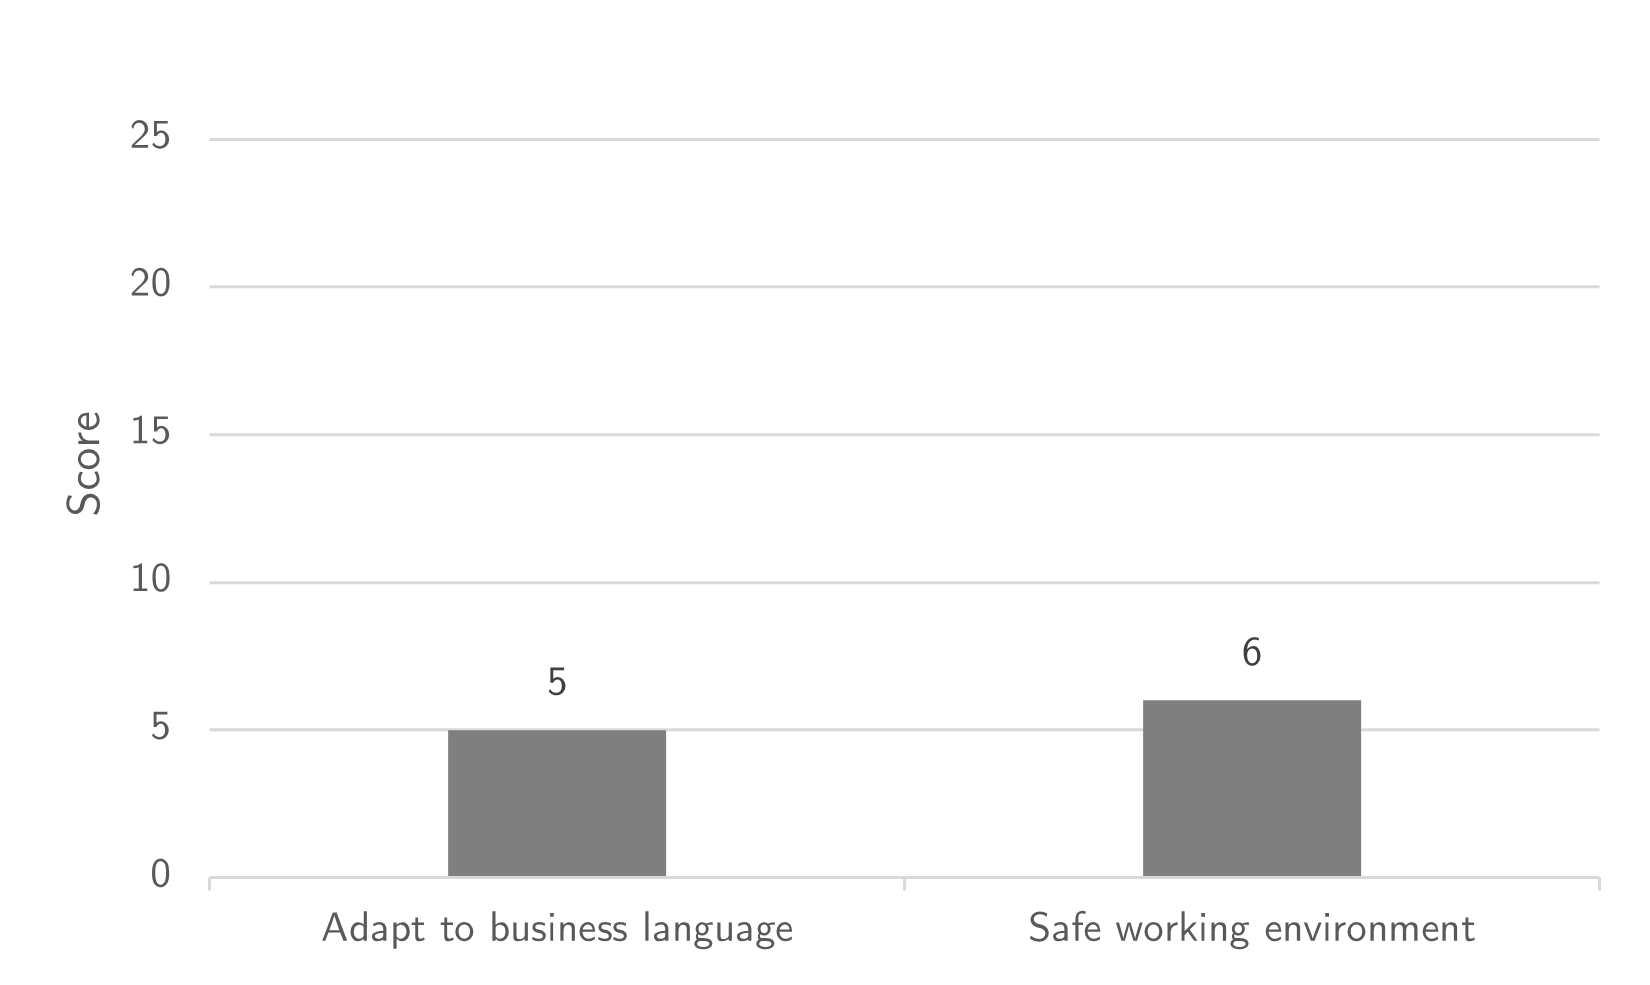
\includegraphics[width=0.475\textwidth]{images/qdanewfindings}
	\caption[QDA new attributes]{QDA new attributes}
	\label{fig:qdanewfindings}
\end{figure}


\subsection{Identified attributes as possible success factors}
\label{sub:identifiedattributesaspossiblesf}
\begin{table}[H]
	\begin{center}
		%\resizebox{\textwidth}{!}{%
			\begin{tabular}{@{}ll@{}}
				\toprule%
				\textbf{Attribute} & \textbf{Category}  \\%
				\midrule%
				\Gls{optionality} & \Gls{amplifyvariety} \\%
				\Gls{nonmonotonicity} & \Gls{amplifyvariety} \\%
				\Gls{selforganisation} & \Gls{amplifyvariety} \\%
				\Gls{failfast} & \Gls{amplifyvariety} \\%
				\Gls{resourcestoinvest} & \Gls{amplifyvariety} \\%
				\Gls{senecabarbell} & \Gls{amplifyvariety} \\%
				\Gls{systeminenvironment} & \acrshort{ea} \Gls{enterpriseecologicaladaptation} \\%
				\Gls{holisticsystemicstance} & \acrshort{ea} \Gls{enterpriseecologicaladaptation} \\%
				\Gls{organisationallearning} & \acrshort{ea} \Gls{enterpriseecologicaladaptation} \\%
				\Gls{environmentallearning} & \acrshort{ea} \Gls{enterpriseecologicaladaptation} \\%
				\Gls{intraorganisationalcoherency} & \acrshort{ea} \Gls{enterpriseecologicaladaptation} \\%
				\Gls{systeminenvironmentcoevolutionlearning} & \acrshort{ea} \Gls{enterpriseecologicaladaptation} \\%
				\Gls{safeworkingenvironment} & New finding \\%
				\Gls{adapttobusinesslanguage} & New finding \\%
				\bottomrule%
			\end{tabular}
		%}
		\caption{Possible success factors identified from interviews}
	\end{center}
\end{table}